\documentclass[9pt,twocolumn,twoside,lineno]{pnas-new}
% Use the lineno option to display guide line numbers if required.
% Note that the use of elements such as single-column equations
% may affect the guide line number alignment. 
\usepackage{subcaption}
\templatetype{pnasresearcharticle} % Choose template 
% {pnasresearcharticle} = Template for a two-column research article
% {pnasmathematics} = Template for a one-column mathematics article
% {pnasinvited} = Template for a PNAS invited submission

\title{Template for preparing your research report submission to PNAS using Overleaf}

% Use letters for affiliations, numbers to show equal authorship (if applicable) and to indicate the corresponding author
\author[a,c,1]{Author One}
\author[b,1,2]{Author Two} 
\author[a]{Author Three}

\affil[a]{Affiliation One}
\affil[b]{Affiliation Two}
\affil[c]{Affiliation Three}

% Please give the surname of the lead author for the running footer
\leadauthor{Lead author last name} 

% Please add here a significance statement to explain the relevance of your work
\significancestatement{Authors must submit a 120-word maximum statement about the significance of their research paper written at a level understandable to an undergraduate educated scientist outside their field of speciality. The primary goal of the Significance Statement is to explain the relevance of the work in broad context to a broad readership. The Significance Statement appears in the paper itself and is required for all research papers.}

% Please include corresponding author, author contribution and author declaration information
\authorcontributions{Please provide details of author contributions here.}
\authordeclaration{Please declare any conflict of interest here.}
\equalauthors{\textsuperscript{1}A.O.(Author One) and A.T. (Author Two) contributed equally to this work (remove if not applicable).}
\correspondingauthor{\textsuperscript{2}To whom correspondence should be addressed. E-mail: author.two\@email.com}

% Keywords are not mandatory, but authors are strongly encouraged to provide them. If provided, please include two to five keywords, separated by the pipe symbol, e.g:
\keywords{Keyword 1 $|$ Keyword 2 $|$ Keyword 3 $|$ ...} 

\begin{abstract}
	Please provide an abstract of no more than 250 words in a single paragraph. Abstracts should explain to the general reader the major contributions of the article. References in the abstract must be cited in full within the abstract itself and cited in the text.
\end{abstract}

\dates{This manuscript was compiled on \today}
\doi{\url{www.pnas.org/cgi/doi/10.1073/pnas.XXXXXXXXXX}}

\begin{document}
%% !Tex root = CS_ORNs.tex

\title{Input gain control confers robust combinatorial \\ odor coding in naturalistic environments}
\date{\today}

\author[1,2]{Nirag Kadakia}
\author[2,3]{Thierry Emonet}
\affil[1]{ Swartz Fellow of Theoretical Neuroscience}
\affil[2]{ Department of Molecular, Cellular, and Developmental Biology, Yale University, New Haven, CT 06511, USA}
\affil[3]{ Department of Physics, Yale University, New Haven, CT 06511, USA}

\maketitle


%%!TEX root = main.tex

\section*{Abstract}

blah.


%%%%%%%%%%%%%%%%%%%%%%%%%%%%%%%%%%%%%%%%%%%%%%%%%%%%%%%%%%%%%%%%%
%%%%%%%%%%%%    		INTRODUCTION	    		%%%%%%%%%%%%%
%%%%%%%%%%%%%%%%%%%%%%%%%%%%%%%%%%%%%%%%%%%%%%%%%%%%%%%%%%%%%%%%%


Animals identify and discriminate odors using olfactory receptors (Ors) expressed in olfactory receptor neurons (ORNs)~\cite{Or_ORNs_maps, buck1991novel}. Individual ORNs, which typically express a single Or~\cite{buck1991novel}, respond to many odorants; likewise, individual odorants activate many distinct ORNs~\cite{friedrich1997combinatorial,hallem_carlson,mosquito_combinatorial_coding,nara2011large}. Odors are  thus believed to be encoded by the distinct patterns of activity they elicit in the sensing periphery
~\cite{malnic1999combinatorial, mosquito_combinatorial_coding, hildebrand1997mechanisms, hallem_carlson, debryune_odor_coding, friedrich1997combinatorial}, patterns then decoded by downstream circuitry into behavioral response ~\cite{early_olfactory_processing}. Ethologically-relevant odors are often mixed together with background ones, and their intensities vary widely as they are carried by the wind ~\cite{odor_backgrounds, murlis_odor_plumes, fluid_dynamics_chemosensory, celani, carde_navigation,celani,srinivas_elife}. How can odors be recognized reliably, despite these variations and confounds? In \textit{Drosophila melanogaster} adult~\cite{hallem_carlson,srinivas_elife} and larvae ORNs~\cite{si2017invariances}, OR-odorant dose response curves exhibit similar Hill coefficients but distinct power-law distributed activation thresholds~\cite{hallem_carlson}~\cite{si2017invariances}, which together with inhibitory odorants~\cite{Cao_Tu_WL} enhance coding capacity~\cite{si2017invariances, Cao_Tu_WL, hallem_carlson}. ORNs project to antennal lobe (AL) glomeruli, where mutual lateral inhibition normalizes population response, helping to maintain the invariance of activity patterns~\cite{lateral_inh_asahina, divisive_normalization}. The sparse degree of synaptic connectivity from the AL projection neurons (PNs) to Kenyon cells in the mushroom body may also enhance neural representations of odor identity, and facilitate compressed sensing decoding schemes~\cite{abbott_axel, litwinkumar, vijay_1}. Concentration-invariant representations of odor identity may also reside in the temporal features of neural response~\cite{stopfer_nat_neuro, stopfer_temporal_model, stopfer_temporal_channel, primacy_coding}. 

Here we examine how time-dependent adaptation at the very front-end of the insect olfactory circuit contributes to the fidelity of odor encoding and decoding. Our theoretical study is motivated by the recent discovery of invariances in the response dynamics of ORNs expressing the co-receptor Orco~\cite{Orco, srinivas_elife, cafaro_WL, cao_WL}. While for some Or-odor combinations, ORN response can exhibit large differences~\cite{montague2011similar}, deconvolution of stimulus dynamics from neuron response produces highly stereotyped filters~\cite{martelli}. Moreover, these filters are invariant to constant odor backgrounds, enabling ORNs to maintain response time independent of odor intensity~\cite{martelli,srinivas_elife}. Similar invariances hold for the entire ensemble of ORNs in \textit{Drosophila} larvae ~\cite{si2017invariances}. These properties stem in part from an apparently universal mechanism of ORN adaptation: gain varies inversely with mean odor concentration according to the Weber-Fechner Law of psychophysics~\cite{weber1996eh,fechner2012elemente,srinivas_elife,cafaro_WL,cao_WL}. This relatively fast adaptation ($\sim 250$ ms) can be traced to feedback mechanisms in odor transduction, upstream of ORN firing machinery~\cite{nagel_wilson_biophysical,cao_WL,cafaro_WL,srinivas_elife}, and the universality of the scaling law suggests its mediation not by odor- or OR-dependent differences, rather by the Orco co-receptor~\cite{Orco,getahun2013insect,getahun2016intracellular}. % SAVE FOR DISCUSSION Phosphorylation sites have been identified on Orco, and some of them have been implicated in desensitization to odors, however over longer timescales (tens of minutes)~\cite{Guo_Smith_review,Guo_Smith}. 

While in a single channel system such as \textit{E. coli} chemotaxis, adaptive feedback via Weber-Fechner's Law robustly maintains sensitivity over concentration changes, the implications for a multiple-channel system -- which combines information from several sensors with overlapping receptive fields  -- is less straightforward. Here we combine a biophysical model of universal ORN adaptive response and neural firing with various sparse signal decoding frameworks to explore how ORN adaptation affects combinatorial coding and decoding of odor signals that span varying degrees of intensity, molecular complexity, and temporal structure. We find that front-end gain modulation with Weber-Fechner scaling helps preserve coding capacity within the non-specifically sensing ORN repertoire and maintains abstract representations of odor identity, beyond what can be achieved by AL divisive normalization alone. As such, this adaptive mechanism promotes the accurate  discrimination of odor signals from strong backgrounds of varying molecular complexity, both in static odor environments and in fluctuating ones. We also investigate the predictions of our model for the \textit{primacy coding} hypothesis  -- that odors are encoded entirely by the few earliest responding ORNs~\cite{primacy_coding, primacy_math}. Our results agree with primacy coding when odor signals are sufficiently simple, though signals composed of more molecular constituents require the recruitment of the full ORN repertoire. Together, our results suggest that despite the broad overlap of ORN tuning curves, a mechanism of front-end adaptation, when endowed with universal Weber-Fechner scaling via the co-receptor Orco, may play a vital role in preserving representations of odor identity in naturalistic odor landscapes.




\section{Results}



%%%%%%%%%%%%%%%%%%%%%%%%%%%%%%%%%%%%%%%%%%%%%%%%%%%%%%%%%%%%%%%%%
%%%%%%%%%%%%    		MODEL DESCRIPTION    		%%%%%%%%%%%%%
%%%%%%%%%%%%%%%%%%%%%%%%%%%%%%%%%%%%%%%%%%%%%%%%%%%%%%%%%%%%%%%%%



\subsection{Model of ORN sensing repertoire}



%%%%%%%%%%%%		TUNING CURVES FIGURE			%%%%%%%%%%%%%

\begin{figure*}[!tb]
	\centering
	\begin{subfigure}[t]{\linewidth}
		\phantomsubcaption
		\label{fig:tuning_curves_a}
	\end{subfigure}
	\begin{subfigure}[t]{0\linewidth}
		\phantomsubcaption
		\label{fig:tuning_curves_b}
	\end{subfigure}
	\begin{subfigure}[t]{0\linewidth}
		\phantomsubcaption
		\label{fig:tuning_curves_c}
	\end{subfigure}
	\begin{subfigure}[t]{0\linewidth}
		\phantomsubcaption
		\label{fig:tuning_curves_d}
	\end{subfigure}
	\begin{subfigure}[t]{0\linewidth}
		\phantomsubcaption
		\label{fig:tuning_curves_e}
	\end{subfigure}
	\begin{subfigure}[t]{0\linewidth}
		\phantomsubcaption
		\label{fig:tuning_curves_f}
	\end{subfigure}
	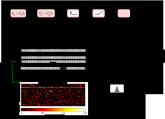
\includegraphics[width=\textwidth]{figures/1_tuning_curves}
	\caption{\footnotesize{
			\textbf{A}~Odor binding model. Or/Orco complexes $\textup{C}_a$ bind odorant molecules $s_i$ comprising stimuli $\textup{S}$. These complexes can stochastically switch between inactive and active states, where the steady-state active fraction is determined by the complex free energy $\epsilon_a(t)$. The activity feeds back on to the free energies with timescale $\tau_a$ to pull the activity to a baseline level $A_{a0}$. ORN firing rates $r_a(t)$ are generated by passing $A_a(t)$ through a linear temporal filter $h(t)$ and a nonlinear thresholding function$f$. 
			\textbf{B}~Odor mixtures are represented by real-valued $N$-dimensional vectors $\mathbf s$, whose components $s_i$ are the concentrations of  the individual molecular constituents  of $\mathbf s$. 
			\textbf{C}~Following (), active binding constants are distributed as a power-law with coefficient $\alpha=0.35$
			\textbf{D}~The maximal firing response of 50 ORNs to the 150-possible monomolecular odors $\mathbf s = s_i$, for the power-law $K^*_{ai}$ distribution in C.
			\textbf{E}~Representative ORN tuning curves, generated by ordering the responses within a single row of the response matrix in D. A diversity of response, mimicking that of~\cite{hallem_carlson}, arises from both the distribution of odorant binding constants $K^*_{ai}$ and the distribution of receptor free energies $\epsilon_a$.}}
	\label{fig:tuning_curves}
\end{figure*}

Odor identification consists of encoding in the sensing periphery followed by decoding in higher-level processing centers of the olfactory circuit. We first examine how front-end adaptation can maintain odor encoding capacity,  by  drawing upon a model of odor-to-ORN firing recently shown to reproduce experimental findings: Weber-Fechner scaling, signal transduction kinetics, and firing rate dynamics of individual \textit{Drosophila} ORNs to fluctuating stimuli ~\cite{srinivas_elife}. Here we generalize this model to a repertoire of $M=50$ ORN types. ORNs house olfactory receptor complexes $\textup{C}_a$, $a=1,...,M$, each consisting of an ORN-specific OR and the universally-expressed olfactory co-receptor Orco, which mediates odor transduction through dendritic localization of and heteromerization with ORs (Fig.~\ref{fig:tuning_curves_a}). These odorant-response functional units interact with odor mixtures, each of which is composed of some combination of $N$ odorant molecules with time-dependent concentrations $s_i(t)$, $i=1,...,N$ (Fig.~\ref{fig:tuning_curves_b}). We choose $N=150$, as this number is sufficiently larger than the size of the sensing repertoire~$M$. Functionally, $\textup{C}_a$ forms a non-selective cation channel whose current is mediated by the strength and nature of bound ligands. We thus model a given complex as stochastically switching between active (channels open) and inactive states, while also being bound or unbound with odorant $i$. The active conformation binds odorant $i$ with higher affinity than the inactive conformation, resulting in distinct dissociation constants, $K^*_{ia}$ and $K_{ia}$, respectively. In steady state, the active fraction $A_a$ of Or/Orco complexes in ORN $a$ can be solved for as (see Methods):
\begin{align}
A_a(t) &= \left(1 + e^{\epsilon_a(t)}\right)^{-1} \nonumber \\
\epsilon_a(t) &= \epsilon_{a, \textup{act}}(t) + \epsilon_{a, \textup{ligand}}(t) \nonumber \\
\epsilon_{a, \textup{ligand}}(t) &= \frac{1 + \sum_i^N s_i(t)/K_{ai}}{1 + \sum_i^N s_i(t)/K^*_{ai}},
\label{eq:steady_state_act_OR}
\end{align}
where $\epsilon_{a, \textup{act}}(t)$ is the free energy cost of $\textup{C}_a$ activation. NAT LOG

Inward currents elicited by activation of the Or/Orco receptor complexes then incite firing activity in ORNs. Following~\cite{srinivas_elife}, we model the Or/Orco-to-ORN transformation with a temporal filter followed by rectifying nonlinearity $f$ (see Methods):
\begin{align}
r_a(t) = f\left(\int h(\tau - t)A_a(t) d\tau\right).
\label{eq:steady_state_firing}
\end{align}
At the single ORN level, this nonlinear-linear-nonlinear framework (Or/Orco activation $\rightarrow$ temporal filter $\rightarrow$ nonlinear rectifier) reproduces Weber Law gain adaptation and signal transduction kinetics, notably the temporal slowdown of the local field potential upon adaptation, along with a complementary speed-up in the firing machinery.





Here $\epsilon_a(t)$ represents the free energy change due to modifications of the Or/Orco complexes by adaptation. Opening of the channels causes an inward current that eventually results in a negative feedback onto $A(t)$. This is modeled minimally by:
\begin{align}
\frac{d\epsilon_a(t)}{dt} = \frac{{A}_{a0} - A_a(t)}{\tau_a}
\label{eq:adaptation_dynamics}
\end{align}
within the finite range $\epsilon_{\textup{L}, a} < \epsilon_a(t) < \epsilon_{\textup{H}, a}$. It has been shown that when properly deconvolved from the stimulus dynamics, the shape of temporal kernels in adult \textit{Drosophila} ORNs is largely odor-independent, though may differ by brief ($\sim$10 ms) odor-dependent delays~\cite{martelli}. Accordingly, we model $h(t)$ by an ORN- and odor-independent double-exponential function, with parameters matched to experiment~\cite{martelli}. We assume that the lower cutoffs $\epsilon_{\textup{L}, a}$ are receptor-dependent and choose them from a normal distribution. This variability ensures that ORNs are activated above quiescence (around 5 Hz) at distinct stimulus levels~\cite{srinivas_elife}.  %The baseline activity level $\bar{A}_a$ is assumed receptor-independent.


%In the absence of activity feedback onto Or/Orco activation (Eq.~\ref{eq:adaptation_dynamics} is zero), 
Diversity among maximal odor-ORN response arises from the distribution of chemical affinities, encapsulated in $K^*_{ai}$. We choose these from a power law distribution ($\alpha = 0.35$), as was recently found across ORN-odor pairs in \textit{Drosophila} larvae (Fig.~\ref{fig:tuning_curves_c}). To mimic the presence of private odors relevant to innate responses, we manually add a high responder ($K^*_{ai} \sim $ small)  to a handful of ORNs; the addition of these private odors did not affect the general findings. Together, the power-law distributed $K^*_{ai}$, receptor-dependent $\epsilon_{\textup{L}, a}$, and invariance in temporal filters, when incorporated into the steady-state model responses Eq.~\ref{eq:steady_state_act_OR}, produce tuning curves mimicking the maximal \textit{Drosophila} ORN responses to many individual odorants~\cite{hallem_carlson} (Fig.~\ref{fig:tuning_curves_d}-\ref{fig:tuning_curves_e}). 



%%%%%%%%%%%%%%%%%%%%%%%%%%%%%%%%%%%%%%%%%%%%%%%%%%%%%%%%%%%%%%%%%
%%%%%%%%%%%%		CODING CAPACITY SECTION			%%%%%%%%%%%%%
%%%%%%%%%%%%%%%%%%%%%%%%%%%%%%%%%%%%%%%%%%%%%%%%%%%%%%%%%%%%%%%%%

\subsection{Concentration-invariant preservation of coding capacity and abstract representations of odor identity}


%%%%%%%%%%%%		CODING CAPACITY FIGURE			%%%%%%%%%%%%%

\begin{figure}[!tb]
	\centering
	\begin{subfigure}[t]{\linewidth}
		\includegraphics[width=\textwidth]{figures/2_coding_representation}
		\phantomsubcaption
		\label{fig:coding_a}
	\end{subfigure}
	\begin{subfigure}[t]{0\linewidth}
		\phantomsubcaption
		\label{fig:coding_b}
	\end{subfigure}
	\caption{\footnotesize{Front-end adaptation maintains information capacity and representations of odor identity across changes in intensity. 
			\textbf{A}~Evolution of mutual information (MI) between odor signals and ORN response, as a function of relative odor concentration. Odor A arrives  at $t_1$ and Odor B (of similar intensity) arrives at $t_2$, where $t_2 - t_1 \gg \tau_A$. MI is plotted for both an unadaptive and adaptive system at times of order of $\tau_A$ following $t_1$ (purple; purple-blue), right before $t_2$ (blue-green), and shortly after $t_2$ (green). 
			%In a  non-adaptive system, mutual information between odor signal and ORN responses, plotted as a function of odor concentration, peaks in a regime of maximum sensitivity with the arrival of one odor (odor A), and shifts to lower concentrations with the arrival of new signals (odor B). An adaptive system pass information over a larger concentration range as ORN responses adapt, eventually  becoming un-informative over time. However, having adapted to the background, it can   then pass the information contained in subsequent signals (lower green plot).
			\textbf{B}~To investigate abstract representations of odor identity in the ORN response, ORN responses are projected from 50 dimensions to 2 dimensions, using nonlinear dimensionality reduction. In the 2D space, distinct odors are plotted as points of distinct colors, and point size represents odor intensity. 
			\textbf{C} In the adaptive system, responses cluster by identity more apparently for an adaptive system (bottom row), than a non-adaptive system (top row), shown here for 10 and 60 sparse odor identities for several concentrations each.}} % Mention that here K1 = 2, K2 = 5}}
	\label{fig:coding}
\end{figure}

To investigate the dependence of encoding capacity on odor concentration, we calculate the mutual information (MI) between odor signals $\mathbf s$ and responses $\mathbf A$ in two sensing systems, one with ORN adaptive feedback (via Eq.~\ref{eq:adaptation_dynamics}) and one without. We consider a simple situation, in which a step of odor A, $\textbf{s}_A$,  turns on at time~$t_1$, persists for some time, and then odor B, $\mathbf s_B$ (a distinct identity) turns on at some later time~$t_2$. For simplicity, we assume that both odors have similar intensities $s_0 = \langle s_i \rangle$ and calculate the MI between the ORN responses $\mathbf {r}_a$ and signals $\mathbf s_A + \mathbf s_B$ at various times after $t_1$, as a function of $s_0$. In the non-adaptive case, MI peaks around the region of maximum sensitivity ($\sim 10^2$ a.u.) after $t_1$ (Fig.~\ref{fig:coding_a}. ORNs are firing at an elevated rate, however, more susceptible to saturation with further odor onsets. Thus, following $t_2$, the maximum shifts leftward as odors of high intensities have saturated the system and cannot pass any more information.

The adaptive system mimics the non-adaptive system at $t_1$,  before adaptation has kicked in (Fig.~\ref{fig:coding_a}). As the activity feeds back onto $\epsilon_a$, the response to higher concentrations passes through the regime of high sensitivity, and the MI peak shifts rightward. Over time, the responses for all signals have reached the baseline firing rate, and the mutual information is mostly eliminated since the firing rate is independent of odor identity. However, having now adjusted its regime of maximum sensitivity to the presence of odor A, the system can respond appropriately to odor B: the MI at $t_2$ is nearly 6 bits across 3 decades of concentration, in contrast to the non-adaptive case. These results suggest that in this multi-channel compressive system, a simple mechanism of universal integral feedback can help maintain sensitivity in changing environments.

We expect that this preservation of information capacity might therefore help maintain  abstract representations of odor identity. To examine such  representations, we project the ORN  response repertoire to a lower dimensional space using t-distributed stochastic neighbor embedding (t-SNE), a nonlinear, local dimensionality reduction technique~\cite{tsne}. Here, each data point is a 50-dimensional vector representing the ORN firing responses to a given odor of a given intensity. Each of these data points is then reduced by t-SNE to  two dimensions (Fig.~\ref{fig:coding_b}). %In Fig. 2B, colors represent odors of distinct identities; sizes represent odors of distinct concentrations. 
Testing this both for a smaller odor repertoire (10 odor identities) and a larger one (60 identities), we find that odors  separate by identity in the adaptive system, while in the unadaptive system, representations  mix among their identity and concentration (Fig.~\ref{fig:coding_b}). Together, these results suggest that at the level of ORN response, front-end adaptation helps maintain representations of odor identity across changes in odor intensity.


%%%%%%%%%%%%%%%%%%%%%%%%%%%%%%%%%%%%%%%%%%%%%%%%%%%%%%%%%%%%%%%%%
%%%%%%%%%%%%    		SIGNAL DECODING      	     %%%%%%%%%%%%
%%%%%%%%%%%%%%%%%%%%%%%%%%%%%%%%%%%%%%%%%%%%%%%%%%%%%%%%%%%%%%%%%


\subsection{Front-end adaptation promotes odor discrimination accuracy in static and fluctuating environments}

Next, we ask how the universal adaptive feedback might contribute to accurate signal reconstruction from ORN responses.  One potentially complicating factor is the disparity between sensor dimension and stimulus dimension: while \textit{Drosophila} only express $\sim 60$ olfactory receptor genes~\cite{olfactory_sensory_map}, the space of aromatic odorants is far greater~\cite{vijay_1}. However, many naturally-occurring odors are comprised of only a small subset of these volatile compounds -- they are sparse in the space of odorants~\cite{vijay_1}. This is suggestive as mathematical results in compressed sensing guarantee the reconstruction of these sparse signals, assuming a sufficiently random response~\cite{CS_donoho, CS_tao, CS_ganguli}. While at this stage of the analysis we use a compressed decoding framework, there is no evidence that this algorithm is being implemented in the \textit{Drosophila} olfactory circuit~\cite{chlovskii_pevlavan}, and we later verify our conclusions with other classification techniques. 

To incorporate the linear framework of compressed sensing into our nonlinear encoding model, we treat the odor encoding process exactly, while approximating the decoding to first order. We denote an odor signal as accurately decoded if both (i) the sparse components are all estimated within some tolerance of their true values, and (ii) the estimates of components not in the odor mixture (``zero" components) are sufficiently low (see Methods). 

To gauge the impact of universal front-end feedback on odor discrimination, we apply this scheme to a static odor mixture containing two sparse odors, which we call the ``foreground" and ``background". We ask how well the foreground can be decoded in the presence of backgrounds of given intensity and molecular complexity. In the unadaptive system, accuracy in the regime of maximum sensitivity is maintained if the background concentration is low enough, but is  compromised as intensity increases (Fig.~\ref{fig:decoding_c}). For higher background concentrations, molecular complexity also has a more damaging effect on decoding accuracy. Finally, for sufficiently strong and complex backgrounds, the foreground is virtually undetectable (top right plot in Fig.~\ref{fig:decoding_c}). The adaptive system is substantially more robust (Fig.~\ref{fig:decoding_d}), although the minimum detectable concentration does increase with background intensity. 

Realistic odor environments are highly variable, with odor concentrations and whiff durations that can span several orders in a short time~\cite{celani}. We next wondered whether a single OR/Orco adaptation timescale ($\tau_{A} \sim 250$ ms~\cite{srinivas_elife}) could promote whiff detection in such environments. We apply our coding framework to a recorded time trace from a photo-ionization detector placed downwind of an odor source (Fig.~\ref{fig:temporal_coding_b}). This trace serves as the odor intensity, to which we randomly assign a sparse identity from the $N$-dimensional odorant space. To investigate discrimination accuracy, we add to this a static background odor signal, and then calculate the percentage of decoded whiffs. Finally, we mimic a finite length of short-term memory, such that only changes in detected odor signal are remembered, and  only for $\tau_{\textup {F}}$ seconds in the past. 

Without ORN adaptation, sufficiently strong backgrounds eliminate whiff-detection ability, irrespective of the complexity of either the foreground or background odor (Fig.~\ref{fig:temporal_coding_c}, green lines). In the adaptive system, this is substantially mitigated, (red lines in Fig.~\ref{fig:temporal_coding_c}) although accuracy does decrease in general with increasing background complexity. Further, accurate whiff detection requires $\tau_{\textup {F}}$ only on the order of $\tau_A$ (darker red lines), indicating that a universal timescale of ORN adaptation promotes detection of naturalistic odor signals amidst confounding backgrounds.


%The signal magnitude was scaled linearly to values applicable to our model framework (a.u.), and we verified that the plume statistics agree with theoretical predictions {~\color{blue} TODO}. 
%For simplicity, we assume that while the sensory response modulates in time, the decoding process itself is instantaneous. We also mimic a finite length of short-term memory, such that only changes in detected odor signal are remembered, and  only for up to $\tau_{\textup {F}}$ seconds in the past. If the signal is static, it will be decoded optimally between $\sim\tau_A$ and $\sim\tau_{\textup{F}}$. For fluctuating environments, we expect that $\tau_{\textup{F}}$ a few times as large as $\tau_A$ should be sufficient in detecting of whiffs of novel odors amid slowly fluctuating or static backgrounds.


%The signal is composed of a series of intermittent whiffs, defined as contiguous regions at which the concentration is above a given value. 



%We first consider the simple case of step stimuli. For shallow steps, odors are rapidly decoded, though slightly more quickly for smaller $\tau_A$ (Fig.~\ref{fig:temporal_coding_a}). This is attributed the recruitment of a sufficient number of ORNs beneath the point of response saturation, such that response adaptation has little effect. For larger steps, decoding accuracy improves gradually as the system adapts at its characteristic timescale. In all cases, the accuracy drops to zero after the forgetting time $\tau_{\textup{F}}$ (here set to $4\tau_A$). 

%{\color {blue} whiffs duration whiffs were not detected or not?}



%%%%%%%%%%%%%%%%%%%%%%%%%%%%%%%%%%%%%%%%%%%%%%%%%%%%%%%%%%%%%%%%%
%%%%%%%%%%%%		SIGNAL DECODING FIGURE			%%%%%%%%%%%%%
%%%%%%%%%%%%%%%%%%%%%%%%%%%%%%%%%%%%%%%%%%%%%%%%%%%%%%%%%%%%%%%%%




\begin{figure*}[!tb]
	\centering
	\begin{subfigure}[t]{\linewidth}
		\includegraphics[width=\textwidth]{figures/3_decoding_temporal}
		\phantomsubcaption
		\label{fig:decoding_a}
	\end{subfigure}
	\begin{subfigure}[t]{0\linewidth}
		\phantomsubcaption
		\label{fig:decoding_b}
	\end{subfigure}
	\begin{subfigure}[t]{0\linewidth}
		\phantomsubcaption
		\label{fig:decoding_c}
	\end{subfigure}
	\begin{subfigure}[t]{0\linewidth}
		\phantomsubcaption
		\label{fig:decoding_d}
	\end{subfigure}
	\caption{\footnotesize{Front-end adaptation promotes accurate sparse odor decoding across concentration changes. 
			\textbf{A}~Odor stimuli produce ORN responses via odor-binding and activation and firing machinery, as described by Eqs.~\ref{eq:steady_state_act_OR}-\ref{eq:steady_state_firing}. Odors are then decoded using compressed sensing by linearizing around a background $s_0$ and minimizing the constrained $L_1$ norm of the odor signal.  Odors are assumed sparse, exhibiting $K$ nonzero components, $K \ll N$. 
			\textbf{B}~Decoding accuracy as a function of odor concentration (a.u.) and odor complexity $K$, for the non-adaptive and adaptive system respectively. 
			\textbf{C}~Decoding accuracy of foreground odors in the presence of background odors. Individual plots the decoding accuracy of the foreground as a function of its intensity and complexity, for the given background odor conditions; the intensity of the background odor increases by column and its complexity by row.
			\textbf{D}~Same as (C), for the adaptive system.}}
	\label{fig:decoding}
\end{figure*}



%In the absence of ORN adaptation, signals are still correctly inferred in a particular regime of mean odor concentration (Fig.~\ref{fig:decoding_b}), corresponding to that of higher coding capacity in Fig.~\ref{fig:coding_a}.  Elsewhere, decoding accuracy is low. Conversely, enforcing Weber-Fechner scaling within the thresholds  $\epsilon_{\textup{L}, a}$ and $\epsilon_{\textup{H}, a}$, coding fidelity is  maintained over a several-fold change in odor intensity (Fig.~\ref{fig:decoding_b}).

%In natural odor environments, accurate olfactory sensing relies on the ability to discriminate multiple odors, which may differ in chemical makeup and intensity. Even if adaptation could preserve decoding accuracy of a single odor amid intensity changes, it is conceivable that a system which adapts to average concentrations alone may well fail for multiple odors of widely differing concentrations. 
%We apply this scheme to the ORN system described above, consisting of 50 Or/Orco complexes interacting with a 150-dimensional odorant space. We assume that number of nonzero odorants comprising the odor, $K$, is small. Note, however, that this still allows for a huge number of distinct odors, e.g. nearly 1 billion for $K= 7$. 




%%%%%%%%%%%%%%%%%%%%%%%%%%%%%%%%%%%%%%%%%%%%%%%%%%%%%%%%%%%%%%%%%
%%%%%%%%%%%%	   	   TEMPORAL CODING                %%%%%%%%%%%
%%%%%%%%%%%%%%%%%%%%%%%%%%%%%%%%%%%%%%%%%%%%%%%%%%%%%%%%%%%%%%%%%





\subsection{Relationship to primacy coding hypothesis}


\begin{figure}[!tb]
	\begin{subfigure}[t]{\linewidth}
		\includegraphics[width=\textwidth]{figures/4_primacy_coding}
		\phantomsubcaption
		\label{fig:primacy_coding_a}	
	\end{subfigure}
	\begin{subfigure}[t]{0\linewidth}
		\phantomsubcaption
		\label{fig:primacy_coding_b}
	\end{subfigure}
	\begin{subfigure}[t]{0\linewidth}
		\phantomsubcaption
		\label{fig:primacy_coding_c}
	\end{subfigure}
	\begin{subfigure}[t]{0\linewidth}
		\phantomsubcaption
		\label{fig:primacy_coding_d}
	\end{subfigure}
	\caption{\footnotesize{\textbf{A} Primacy coding posits that only the first $p$ ($p < N$) active glomeruli are responsible for encoding odor identity. \textbf{B} Decoding accuracy as a function of the number of active ORNs (firing rate $>$ 15 Hz), for different odor complexities. \textbf{C} Number of active ORNs required to fully decode odor signals of varying odor intensity and complexity. \textbf{D} Shift in time to achieve accurate odor identification, as a function of the intensity of odor steps, for various odor complexities (various green-blue lines).
	}}
	\label{fig:primacy_coding}
\end{figure}



An intriguing emergent hypothesis, ``primacy coding,"  posits that odor identity is encoded entirely by the set (but not order) of the $p$ earliest responding glomeruli, called ``primacy sets" of order $p$ (Fig.~\ref{fig:primacy_coding_a}). Primacy sets would in principle comprise a concentration-invariant representation of odor identity. In our framework, odors are decoded via information passed simultaneously from all 50 ORNs. However, some of this information may be redundant, whereby a set of earliest active ORNs are sufficient for odor recognition; if so, our theory would generate predictions in agreement with primacy coding. To test this, we consider a steep sigmoidal stimulus with half-max slope of $1/50$ ms$^{-1}$, as in Fig.~\ref{fig:primacy_coding_a}. We calculate the decoding accuracy as a function of time, and plot in Fig.~\ref{fig:primacy_coding_b} the accuracy as a function of number of active ORNs, which increases monotonically as the signal rises (Fig.~\ref{fig:primacy_coding_a}). To illustrate how the recruitment of ORNs incrementally improves odor signal recognition, we allow for partial accuracy by calculating  the percentage of correctly decoded individual odor components.

For sufficiently simple odors, our results are indeed in accordance with primacy coding: the set of earliest responding neurons fully account for the odor identity ($K=1, 3, 5$ plots in Fig.~\ref{fig:primacy_coding_b}). Though all ORNs eventually activate as the stimulus increases, the latter responders confer no further information in odor recognition. As expected, the active ORN subset comprising the primacy set is distinct for each odor,   {\color{blue} Show that recruited ORNs are all distinct}. We do find, however, that for more complex odor mixtures, the full ORN repertoire must be active for  accurate decoding ($K=7, 9$ plots in Fig.~\ref{fig:primacy_coding_b}), a result that holds across odor  odor concentrations (Fig.~\ref{fig:primacy_coding_c}). In this regime, there can  be no primacy code, since a primacy set consisting of the full ORN repertoire would encode only a single odor. Conversely, our framework can decode the odor for a maximal primacy set since it utilizes not just the identity of the active ORNs, but also their individual firing responses. Primacy coding also predicts that for stronger stimuli, behavioral responses shift earlier in time, since the primacy set is activated quicker. We calculate this time shift and find that it rises monotonically with odor intensity over a decade of concentrations.  %The timescale is on the same order as those measured (18 ms measured; here 60 ms), though the model organisms are different, so this may not be particularly meaningful. 

Primacy sets are inherently concentration-invariant. But to what extent are they conserved among varying environmental conditions, such as persistent background odors? ORNs that have adapted their gain in response to a background odor could in principle be pushed out of the primacy sets of a novel odor due to reduced sensitivity. To test this, we calculated the primacy sets for 1000  sparse odor mixtures atop a static background of a low and high intensity, comparing their primacy sets for each mixture. Primacy sets of sufficient size ($p \gtrapprox 8$) are almost entirely preserved across odor concentration, indicating that primacy coding, if true, would benefit from universal ORN  adaptation in maintaining concentration-invariant odor representations in confounding environments. (Figure forthcoming)


Together, these results suggest that front-end adaptation, in concert with the compressed sensing paradigm, are largely in agreement with the predictions of the primacy coding hypotheses. Our framework also provides the testable prediction that primacy coding may break down for more complex odor mixtures.

\subsection{Cooperative effects of ORN adaptation and  downstream normalization}


\begin{figure*}[!tb]
	\begin{subfigure}[t]{\linewidth}
		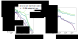
\includegraphics[width=\textwidth]{figures/5_downstream}
		\phantomsubcaption
		\label{fig:downstream_a}	
	\end{subfigure}
	\begin{subfigure}[t]{0\linewidth}
		\phantomsubcaption
		\label{fig:downstream_b}
	\end{subfigure}
	\begin{subfigure}[t]{0\linewidth}
		\phantomsubcaption
		\label{fig:downstream_c}
	\end{subfigure}
	\begin{subfigure}[t]{0\linewidth}
		\phantomsubcaption
		\label{fig:downstream_d}
	\end{subfigure}
	\caption{\footnotesize{\textbf{A} Odors of various identity and intensity are encoded by the ORN sensing repertoire (with Weber Law adaptation), which sends signals to glomeruli in the AL, where they are further normalized via lateral inhibition. AL projections neurons then send divergent connections to Kenyon cells in the MB. A linear classifier trains the output of the MB, classifying them either by valence or by odor identity. \textbf{B} Accuracy of binary classification by odor valence, as a function of the number of distinct odor identities classified by the trained network (concentrations span 4 orders of magnitude), in systems with only ORN adaptation, only divisive normalization, both or neither. \textbf{C} Same as (B), but with concentrations spanning only 1 order. \textbf{D}, same as (B) but now classifying in distinct classes by their identity.}}
	\label{fig:downstream}
\end{figure*}


Lateral inhibition among antennal lobe glomeruli normalizes ORN responses prior to their projections to the mushroom body~\cite{lateral_inh, lateral_inh_asahina}. This inhibition obeys a type of divisive gain control, normalizing each input by the sum of ORN activity~\cite{divisive_normalization}. To what extent does Weber Law adaptation in the olfactory periphery act in tandem with (or counteract) this downstream normalization to maintain odor representations? To investigate this, we extended our ORN encoding model by adding uniglomerular connections from ORNs to the antennal lobe, followed by sparse, divergent connections to 2500 Kenyon cells (KCs) in the mushroom body~\cite{memory_review, litwinkumar, abbott_axel} (Fig.~\ref{fig:downstream_a}). Divisive normalization in the AL was modeled via~\cite{divisive_normalization}:
\begin{align}
r_{\textup{PN}, a}(t) = \frac{r_a(t)^{1.5}}{\sigma^{1.5} + r_a(t)^{1.5} + (\gamma\sum_b^Mr_b(t))^{1.5}}
\end{align}
%then training and testing KC activity patterns by training
We then quantified decoding accuracy by training and testing a binary linear classifier on the KC activity output of  many sparse odors of distinct intensity and identity,  each randomly categorized as appetitive or aversive. Odor signals of the same identity but differing intensity were assigned the same valence (Fig.~\ref{fig:downstream_a}). We trained the classifier on $p$ sparse odor identities at intensities chosen randomly over 4 orders of magnitude, then tested the classifier accuracy on the same odor identities but of differing concentrations. 

Classification accuracy degrades to chance level as the number of distinct odor identities $N_{\text ID}$ becomes very high (Fig.~\ref{fig:downstream}). When acting alone, either divisive normalization or ORN adaptation can mitigate this, although the effect of ORN adaptation is stronger (Fig.~\ref{fig:downstream_b}). When both are active, accuracy improves further, suggesting that these distinct adaptive transformations may act jointly at different stages of neural processing to preserve representations of odor identity.  If odors are instead chosen from a narrower intensity range, performance improves without either adaptive mechanism at play~(Fig.~\ref{fig:downstream_c}). Interestingly, if we train the classifier to distinguish odors by their distinct identity using multiclass categorization (Fig.~\ref{fig:downstream_a}), we find that the benefits conferred by divisive normalization do not appear until $p$ is substantial, with accuracy below $65\%$ for $N_{\text ID} > 50$ (Fig.~\ref{fig:downstream_d}). On the other hand, with ORN adaptation accuracy remains above $85\%$ for $N_{\text ID}$ as high as 1000. Together, this indicates that front-end adaptation plays a key role in maintaining odor identity representations, before they are further normalized and diverged in downstream processing. In some categorization tasks, subsequent normalization can further preserve these representations.

%{\color{blue} Code with temporal sequence of odors, not strength or subset? Each vector is  the sequence of temporal activation -- does adaptation help? }

%%%%%%%%%%%%%%%%%%%%%%%%%%%%%%%%%%%%%%%%%%%%%%%%%%%%%%%%%%%%%%%%%
%%%%%%%%%%%%	   	        DISCUSSION                %%%%%%%%%%%
%%%%%%%%%%%%%%%%%%%%%%%%%%%%%%%%%%%%%%%%%%%%%%%%%%%%%%%%%%%%%%%%%



\section{Discussion}

{\color {blue}-- also don't forget to mention that the odor-receptor  interactions are nonlinear and that saturation is important in this case -- also many odors}

%Stopfer -- information in each pulse enough (small 50s bins) is enough to classify odors . Go further here and say that even in odor connfounds and complex odors, same conclusion follows. maybe do this for temporal presentation, not odor reconstruction, just order?

We investigate, through theory and computations, the implications of recent experimental evidence for a universal mechanism of input gain control in \textit{Drosophila} olfactory receptor neurons. We argue that this mechanism, Weber's Law of psychophysics, plays a key role in preserving neural representations of odor identity at the front-end of the olfactory pathway, prior to further transformations downstream. Tnput gain control also acts jointly with normalization in the antennal lobe, implicating the importance of signal transformations at multiple steps in the circuit. We support our conclusions using both a decoding scheme that fully reconstructs odor signals from neural response, and a classification scheme that categorizes odors by identity or valence. We find that input gain control is especially central to the discrimination of fluctuating odor signals from potentially saturating odor backgrounds. For single odorants or simple odor mixtures, our results are also consistent with the primacy coding hypothesis, that signals may be fully encoded by the primacy set of earliest activating glomeruli. %Further, the primacy set is preserved even when background odors are 

\subsection{Universal front-end adaptation in multi-channel sensory systems}

In living systems, sensory adaptation ensures that responses remain in regimes of maximum sensitivity, increasing their effective dynamic range~\cite{adaptation_fairhall, adaptation_nagel, laughlin, deweese_adaptation}. Viewing sensory systems as input/output machines, the role of adaptation is therefore to maintain information capacity in dynamic environments~\cite{information_theory_adaptation}. Doing so requires matching sensory response to attributes of the environment, either by adapting to specific stimuli or to stimuli statistics~\cite{adaptation_fairhall}. In a single-channel system such as bacterial chemotaxis, information capacity is increased by matching the midpoint of the nonlinear dose-response curve, where sensitivity is highest, to mean ligand concentration~\cite{information_theory_adaptation}. This is enacted in a robust and dynamic way, through a feedback loop from the activity output of the pathway onto proteins dictating receptor sensitivity~\cite{robustness_barkai, robustness_alon}. It is hypothesized that an analogous feedback loop exists in olfactory receptor neurons, from Orco-mediated Or channel activity onto the free energy of receptor activation~\cite{srinivas_elife}. This mechanism appears to act identically across ORNs, and because olfactory receptive fields are highly overlapping, raises questions about its efficacy in complex environments: adaptation to one odor could adversely affect identification of a new odor if the latter excites some but not all of the same ORNs. Our results show that this universal mechanism of front-end gain control does help to preserve combinatorial representations of odor identity, despite these broad overlaps. 

While Weber-Fechner gain control operates at the level of individual ORNs, lateral inhibition in antennal lobe glomeruli mixes signals among all ORNs~\cite{divisive_normalization}. We find that olfactory circuits exhibiting both of these adaptive mechanisms outperform systems containing one alone. 
Combinatorial coding, therefore, benefits both from the separate adaptation of individual single sensory neurons, as well as the normalization of aggregated response. It is notable that both Weber-Fechner adaptation and divisive normalization modulate the location of maximal sensitivity rather than the scale of absolute activity -- they move dose-response curves horizontally, rather than stretching them vertically. They are both mechanisms of input gain control rather than response gain control. {\color{blue} Such input mechanisms are common to other models, sensory ssytems, etc... (...la)}. 

Other mechanisms in the sensory periphery likely play a role in maintaining neural representations of odor identity. ORNs that contain both excitatory and inhibitory responses to odorants can increase information capacity by exploiting bidirectionality of response~\cite{Cao_Tu_WL}. %Our framework uses the power law-distributed $K^*_{\textup D}$ as measured in from \textit{Drosophila} larvae, but one cannot find 
Antagonism among odorants, in which multiple odorants compete for common ORN binding sites, could help maintain the sparsity of glomerular activation, provided that binding and activation strengths are uncorrelated~\cite{reddy2017antagonism}. This mechanism requires odor-specific activation processes, i.e. G protein-coupled, cAMP-mediated transduction as in mammalian olfaction (Spehr, Munger 2009). We rely instead on experimental evidence for non-ORN-specific and non-odor-specific dynamic gain control acting via the universally expressed co-receptor Orco (Or83b)~\cite{srinivas_elife}.  %it is plausible that ion channel dynamics carry odor-specific dependencies we have not accounted for here. {\color {blue} blah..}. 

\subsection{Odor identification in natural odor environments}

Our results are relevant for understanding combinatorial odor coding in naturalistic odor environments. Dynamic gain control acting on a universal timescale of $\sim 250$ ms allows the of determination of odor identity from single whiffs, particularly when these whiffs are mixed among static backgrounds. The gains afforded by rapid ORN adaptation increase with the strength and complexity of the background odor, suggesting the involvement of ORN adaptation in odor discrimination. %Further, categorizing odors via learned associations, but reconstruction odor signals in their entirety. While we make no claims that olfactory circuits seeks such a reconstruction, the anatomical features and mechanisms of the olfactory periphery and circuit are sufficient to do so.
Our results indicate that despite the generality in the adaptive mechanism (which also acts on a universal timescale), odor coding capacity and decoding fidelity are greatly enhanced. 


%Though less rare in laboratory settings, which focus on discernment of molecularly simple, static odor signals, odor discrimination is ubiquitous in the natural world. 
Indeed, {\color {blue} Add discrimination papers here}.

%\subsection{power law}


%\subsection{How to discriminate intensities?}
%Both Weber ORN adaptation and divisive gain control normalize out signal intensity, thus maintaining concentration-invariant odor representations. 

\subsection{Spatiotemporal odor coding and the primacy hypothesis}

Previous studies implicate not only the combination of active ORNs but also their distinct temporal patterns as signatures of odor identity~\cite{stopfer_temporal_model, multiple_timescales_stopfer, stopfer_nat_neuro, stopfer_temporal_channel}. ORNs modeled on observed features of these temporal patterns form distinct trajectories in low-dimensional projections, projections which cluster by odor identity, much as we have found here (Fig.~\ref{fig:coding_b}). Though we do explicitly utilize the temporal history of neural firing in our decoding schemes, the transmission of information over time is implicit in this framework. Because the strength of ORN feedback onto receptor complex activation
% $\epsilon_a(t)\tau_A = \int^t_{-\infty} dt(A_a(t) - A_{0})$, 
depends on each ORN's unique tuning curve, odor signals are naturally formatted into temporal patterns that are both odor- and ORN-specific. The response repertoire at a given time is shaped by response history via integral feedback, and the short forgetting timescales, $\tau_{\textup F} \sim \tau_{\textup A} ~ \sim 250$ ms, suggest that only information in brief temporal windows is required for accurate odor identification, consistent with previous findings~\cite{stopfer_nat_neuro}. On the other hand, the classification scheme we employ here (Figs.~\ref{fig:downstream}) could ...



Primacy coding also exploits the temporal sequence of glomeruli activation, but in a coarser sense: while the order of ORN activation defines the primacy set, within this set the order is immaterial. We too find that information contained in a primacy subset of the full ORN repertoire can be sufficient for accurate reconstruction of simple odor mixtures. An extension we find, in support of the primacy coding hypothesis, is that primacy sets are also preserved even in the presence of potential confounds such as background odors. 




\iffalse
Coding with temporal in binary signal? -- not sure how to make linear response though.

Asahina paper
Mention mixtures
redo classification tasks with simple mixtures?
Nemenman paper
https://journals.plos.org/ploscompbiol/article?id=10.1371/journal.pcbi.1006175
\fi

%%%%%%%%%%%%%%%%%%%%%%%%%%%%%%%%%%%%%%%%%%%%%%%%%%%%%%%%%%%%%%%%%
%%%%%%%%%%%%	   	           METHODS                %%%%%%%%%%%
%%%%%%%%%%%%%%%%%%%%%%%%%%%%%%%%%%%%%%%%%%%%%%%%%%%%%%%%%%%%%%%%%




\section{Methods}

{\color {blue} This section needs to be redone}

\subsection{Stochastic odor-receptor binding model}

We model an odor as an $N$-dimensional vector $\mathbf s = \langle s_1,...,s_N\rangle$, where $s_i > 0$ are the concentrations of individual volatile molecules (odorants) comprising the odor. In addition, we assume that the odors are sparse in the space of odorants, so only $K$ components of $\mathbf s$ are nonzero, where $K \ll N$. The olfactory sensory system is modeled as a collection of $M$ distinct Or/Orco complexes, each of which can be bound with any one of the odorant molecules, and can be either active (firing) inactive (quiescent). We only consider competitive binding, so a complex is bound with one odorant at most. With $N$ possible odorants, receptor $a$ resides in one of $2N+2$ possible states, \{$R_a$, $R^*_a$, $R_a$-$s_i$, $R^*_a$-$s_i$\}, indicating receptors that are unbound/inactive, unbound/active, inactive/bound to odorant $i$, and active/bound to odorant $i$, respectively. We set $N = 150$ and $M = 50$ throughout.

In the mean-field limit, the binding dynamics of these $2N + 2$ states are described by the master equations:

\begin{align}
\frac{d[R_a\text{-}s_i]}{dt} &= k^+_{ia}s_i[R_a] - k^-_{ia}[R_a\text{-}s_i] \label{eq:Meq_inactive_bind_rate}\\
\frac{d[R^*_a\text{-}s_i]}{dt} &= k^{*+}_{ia}s_i[R^*_a] - k^{*-}_{ia}[R^*_a\text{-}s_i],
\label{eq:Meq_active_bind_rate}
\end{align}
when receptor $R_a$ is either inactive (Eq.~\ref{eq:Meq_inactive_bind_rate}) or active (Eq.~\ref{eq:Meq_active_bind_rate}). Further, transitions between inactive and active states are described in the mean limit via:
\begin{align}
\frac{d[R_a]}{dt} &= w^{\text{u}+}_a [R_a] - w^{\text{u}-}_a [R^*_a] \label{eq:Meq_unbound_active_rate}\\
\frac{d[R^*_a\text{-}s_i]}{dt} &=  w^{\text{b}+}_{ia} [R_a\text{-}s_i] - w^{\text{b}-}_{ia}  [R^*_a\text{-}s_i],
\label{eq:Meq_bound_active_rate}
\end{align}
when receptor $R_a$ is either unbound (Eq.~\ref{eq:Meq_unbound_active_rate}) or bound (Eq.~\ref{eq:Meq_bound_active_rate}). The corresponding disassociation constants in terms of the binding transition rates are:


\begin{align}
K_{ia} = \frac{k^-_{ia}}{k^+_{ia}} \nonumber \\
K^*_{ia} = \frac{k^{*-}_{ia}}{k^{+*}_{ia}} 
\label{eq:Kd}
\end{align}

Following~\cite{srinivas_elife}, we assume that in steady state, the active firing state of an Or/Orco complex is energetically suppressed from the inactive state through corresponding Boltzmann factors:

\begin{align}
\frac{[R^*_a]}{[R_a]} &= \frac{w^{\text{u}+}_a}{w^{\text{u}-}_a} \equiv e^{-\epsilon_a} \label{eq:epsilon_unbound} \\
\frac{[R^*_a\text{-}s_i]}{[R_a\text{-}s_i]} &= \frac{w^{\text{b}+}_{ia}}{w^{\text{b}-}_{ia}} \equiv e^{-\epsilon^{\text b}_{ia}}.\label{eq:epsilon_bound}
\end{align}
These energies are related through detailed balance, which we assume. Applying detailed balance to a given 4-cycle 
\begin{align}
R_a \rightarrow R_a^* \rightarrow R_a^*\text{-}s_i \rightarrow R_a\text{-}s_i \rightarrow R_a
\end{align}
gives
\begin{align}
\frac{w^{\text{u}+}_a}{w^{\text{u}-}_a}\frac{k^{*+}_{ia}}{k^{*-}_{ia}}\frac{w^{\text{b}-}_{ia}}{w^{\text{b}+}_{ia}}\frac{k^{-}_{ia}}{k^{+}_{ia}} \equiv 1,
\label{eq:detailed_balance}
\end{align}
which, in conjunction with Eqs.~\ref{eq:Kd}, \ref{eq:epsilon_unbound}, and \ref{eq:epsilon_bound}, gives
\begin{align}
\epsilon_{ia}^{\text b} = \epsilon_a + \ln\left[\frac{K^*_{ia}}{K_{ia}}\right].
\label{testing_equation}
\end{align}
Assuming the binding dynamics are fast, then the probability that receptor $a$ is bound by ligand~$i$ when inactive and active can be derived from  Eqs.~\ref{eq:Meq_inactive_bind_rate} and \ref{eq:Meq_active_bind_rate} as
\begin{align}
p^{\text b}_{ia} = \frac{s_i/K_{ia}}{1 + \sum_j^Ns_j/K_{ja}} \label{eq:bound_prob_ai_inactive} \\
p^{\text b, *}_{ia} = \frac{s_i/K^*_{ia}}{1 + \sum_j^Ns_j/K^*_{ja}} \label{eq:bound_prob_ai_active}.
\end{align}
The average  activity $A_a$ of complex $a$ is the likelihood that the complex is active, unbound or unbound (equivalantly, the proportion of Or/Orco complexes in a given ORN that are active):
\begin{align}
A_a = \frac{[R^*_a] + \sum_i^N[R^*_a\text{-}s_i]}{[R^*_a] + \sum_i^N[R^*_a\text{-}s_i] + {[R_a] + \sum_i^N[R_a\text{-}s_i]}}.
\end{align} 
Using the master equations between active and inactive states Eq.~\ref{eq:Meq_unbound_active_rate} and \ref{eq:Meq_bound_active_rate}, this activity obeys the master equation
\begin{align}
\frac{dA_a}{dt} &= w^+_a(1 - A_a) + w^-_aA_a
\label{eq:dadt}
\end{align}
with effective transition rates
\begin{align}
w^+_a &= \sum_i^Np^{\text b}_{ia} w^{\text u +}_{ia} + p_{a}w^{\text u}_a 
\end{align}
and analogously for $w_a^-$. Setting Eq.~\ref{eq:dadt} to zero gives the steady state average activity level of ORN $a$:
\begin{align}
A_a = \left(1 + e^{\epsilon_a}\frac{1 + \sum_i^N s_i/K_{ia}}{1 + \sum_i^N s_i/K^*_{ia}}\right)^{-1}. \tag{\ref{eq:steady_state_act}}
\end{align}

\subsection{Generation of binding matrices $K^*_{ia}$}
TODO

\subsection{Compressed sensing decoding of ORN response}
We decode ORN responses to infer odor signal identities using an abstraction intended to mimic the neural computations underlying odor identification in the \textit{Drosophila} mushroom body. While we make no assumptions that the compressed sensing (CS) algorithm (or one like it) is being utilized in actuality, this framework nonetheless informs our understanding of how the neural representation of odor identity is maintained or lost when passed through a distributed ORN repertoire. In this sense, CS is somewhat of an upper bound on how well a real neural computation might perform in decompressing ORN responses.

We assume that ORN firing rates are linear in the Or/Orco complex activity; for simplicity we let this transform be the identity. Though subsequent neural circuitry, particularly from the glomeruli in the AL to the Kenyon cells in the MB further mix and scramble these responses, we focus here on the information transfer at the sensory periphery alone. In any case, as demonstrated previously~\cite{vijay_1}, we expect that these neural computations would only improve the representation of neural identity, so we expect no negative ramifications for our findings.

CS addresses the problem of determining a sparse signal from a set of linear measurements, when the number of measurements is less than the signal dimension. Specifically, it is a solution to 
\begin{align}
\mathbf y = \mathbf R\mathbf s,
\label{eq:CS_constraints}
\end{align} where $\mathbf s \in \mathbb{R}^N$ and $\mathbf a\in \mathbb{R}^M$ are vectors of signals and responses, respectively, and $\mathbf R$ is the measurement matrix. Since measurements are fewer than signal components, then $M < N$, whereby $\mathbf R$ is wide rectangular and so Eq.~\ref{eq:CS_constraints} cannot be simply inverted to produce $\mathbf s$. The idea of CS is to utilize the knowledge that $\mathbf s$ is sparse, i.e.g only $K$ of its components, $K \ll N$ are nonzero. Both the measurements and sparsity are thus combined into a single constrained optimization routine:
\begin{align}
\hat s_i = \textup{argmin} \sum_i^N |s_i| \quad \textup{such that } \mathbf y = \mathbf R\mathbf s
\label{eq:CS}
\end{align}
where $\hat s_i$ are the optimal estimates of the signal components and the sum, which is known as the $L_1$ norm of $\mathbf s$, is a natural metric of sparsity. 

Importantly, the $L_1$ norm is a convex operation and the constraints are linear, so the optimization has a unique global minimum. To incorporate the nonlinear response of our encoding model into this linear framework, we assume that the responses are generated through the full nonlinear steady state response, Eq.~\ref{eq:steady_state_act}, but that the measurement matrix needed for decoding uses a linear approximation of this transformation.  Expanding Eq.~\ref{eq:steady_state_act} around $s_0 = s_i - \Delta s_i$ gives
\begin{align}
A_a &\approx A_{a, 0} + \Delta A_a \label{eq:CS_act_approx} \\
\Delta A_a &= \sum_i^NR_{ia}\big|_{s_0}\Delta s_i \label{eq:CS_dAct_approx}\\
A_{a, 0} &= \frac{\sum_1^N s_0/K_{ia}^*}{\sum_1^N s_0/K_{ia}^* + e^{\epsilon_a}} \label{eq:CS_act0_approx} \\
R_{ia}\big|_{s_0} &=  \frac{e^{\epsilon_a}/K_{ia}^*}{(\sum_i^Ns_0/K_{ia}^* + e^{\epsilon_a})^2},
\label{eq:CS_gain_approx}
\end{align}
where we work in the approximation $K^*_{ia} \ll~s_0 \ll K_{ia}$. We assume that the neural system has access to the linearized response, Eq.~\ref{eq:CS_gain_approx}, but must infer the excess signals $\Delta s_i$ from the excess activity $\Delta A_a$. Corresponding to the CS framework, therefore, $\Delta \mathbf {A} \rightarrow \mathbf y$, $\Delta \mathbf s \rightarrow \mathbf s$, and $R_{ia}\big|_{s_0} \rightarrow \mathbf R$. We optimize the cost function in Eq.~\ref{eq:CS} using sequential least squares programming, implemented in Python through using the scientific package SciPy.

\subsection{Or/Orco  energies of activation $\epsilon_a$ and enforcement of Weber's Law}
Free energies are considered receptor-independent throughout, with the exception of dynamically adaptive system in a temporal odor environment (Figs.~\ref{fig:temporal_coding} and \ref{fig:temporal_coding_2}). To enforce Weber's Law, we assume the receptor activities feed back onto $\epsilon_a$ through the free energies. For the static case, adaptation is perfect, whereby Or/Orco activities are pegged to perfectly adapted values $\bar {A}_{a}$. Incorporating this into Eq.~\ref{eq:steady_state_act}, and assuming  $K^*_{ia} \ll s \ll K_{ia}$, gives
\begin{align}
\bar \epsilon_a &= \ln\left(\frac{1-\bar {A}_{a}}{\bar {A}_{a}}\right) + \ln\left(\sum_i^N\frac{s_i}{K_{ia}^*}\right).
\label{eq:adapted_epsilon}
\end{align}
Assuming that the excess signals are small, $\Delta s_i < s_0$, this gives 
\begin{align}
\epsilon_a \approx \ln(s_0) + \epsilon_{a, 0},
\label{eq:WL_approx}
\end{align} 
where $\epsilon_{a, 0}$ are receptor-dependent constants. In the static case, we choose these constants such that $\epsilon_{a}$ in both adaptive and non-adaptive systems are equivalent, equal to $\epsilon_{\text {L}}$, at a given low concentration, $s_{0, \text L}$.  Below this concentration, we assume adaptation is not in effect, so $\epsilon_a  = \epsilon_{\text {L}}$.  

It is important to note that while the linearized gain Eq.~\ref{eq:CS_gain_approx} utilized by the decoding algorithm appears to rely on $\epsilon_a$, by the above argument $\epsilon_a$ can in principle be determined by firing rates alone. That is, $\epsilon_a$ is inferred in time through integration of Eq.~\ref{eq:WL_dynamics}, which relies only on the current ORN activity.


\begin{table*}[!tb]
	\centering
	{\small
		\begin{tabular}{ccccccccccccccc}
			Figure & $N$& $M$ & $K$ & $\mu_{a, \text L}$ & $\mu_{a, \text H}$ & $\nu_{a, \text L}$ & $\nu_{a, \text H}$ & $\epsilon_{a, 0}$ & $\epsilon_{\text {L}}$  & $\epsilon_{\text {H}}$  & $s_{0, \text L}$ & $s_k$ & $s_{k, \text F}$\\[0.1cm]
			
			\hline \\[-0.2cm]
			\smallskip
			
			\ref{fig:tuning_curves_c} & 200 & 40 & 6 & $2\cdot 10^{-4}$ & $10^{-3}$ & $10^{-2}$ & 1.0 & 5.4 & 5.4 & 10  & - & $ \mathcal N\left(\frac{s_0}{5}, \frac{s_0}{15}\right)$ & --\\
			
			\ref{fig:decoding_a} & 100 & 50 & 7 & 0.5 & 0.5 & 0.8 & 0.8 & 5.4 & 3.1 & 10  & $10^{-1}$ & $ \mathcal N\left(\frac{s_0}{3}, \frac{s_0}{15}\right)$ & -- \\
			
			\ref{fig:decoding_b} & 100 & 50 & 7 & 0.5 & 0.6 & 0.6 & 0.9 & 5.4 & 3.1 & 10 & $10^{-1}$ & $ \mathcal N\left(\frac{s_0}{3}, \frac{s_0}{15}\right)$ & ---\\
			
			\ref{fig:decoding_c} & 100 & 50 & 7 & 0.5 & 0.6 & 0.6 & 0.9 & 5.4 & 3.1 & 10 & $10^{-1}$ & $ \mathcal N\left(\frac{s_0}{3}, \frac{s_0}{15}\right)$ & -- \\
			
			\ref{fig:signal_discrimination_a}-\ref{fig:signal_discrimination_h} & 100 & 50 & 7 & 0.5 & 0.6 & 0.6 & 0.9 & 5.4 & 3.1 & 10 & $10^{-1}$ & $ \mathcal N\left(\frac{s_0}{3}, \frac{s_0}{15}\right)$ & $ \mathcal N(1, \frac{1}{5})$ \\
			
			\ref{fig:temporal_coding} & 100 & 50 & 7 & 0.5 & 0.6 & 0.6 & 0.9 & -- & -- & -- & $10^{-2}$ & $ \mathcal N\left(\frac{s_0}{3}, \frac{s_0}{9}\right)$ & -- \\
			
			\ref{fig:temporal_coding_2} & 100 & 50 & 7 & 0.5 & 0.6 & 0.6 & 0.9 & -- & -- & -- & $10^{-2}$ & $ \mathcal N\left(\frac{s_0}{3}, \frac{s_0}{9}\right)$ & -- \\
		\end{tabular}
	}
	\caption{Parameters for simulations in all of the figures.}
	\label{tab:params}
\end{table*}



\subsection{Odor signals}
Odor signals $\mathbf s$ are $N$-dimensional vectors presumed sparse whereby only $K$ components, $s_k$ are nonzero,  $K~\ll~N$. The magnitudes of the nonzero components $s_k$ are denoted $s_0 + \Delta s_k$. Here, $\Delta s_k$ is a random vector, while $s_0$ is both the center of linearization and, in the case of the adaptive system, the value dictating the strength of adaptive feedback $\epsilon_a\sim\ln\langle s_0 \rangle$. 

All the signal intensities are in arbitrary units, as they can be scaled to any range by a corresponding shift in the scales of $K_{ia}$ and $K^*_{ia}$.

\subsection{Dynamic adaptation}

Dynamic adaptation is enforced through
\begin{align}
\frac{d\epsilon_a(t)}{dt} &= \frac{1}{\tau_a}\left[A_a - \bar {A}_{a}\right].
\tag{\ref{eq:WL_dynamics}}
\end{align}
The perfectly adapted activity levels $\bar {A}_{a}$ are determined by evaluating Eq.~\ref{eq:steady_state_act} at a given odor intensity, $s_{0, \text{L}}$, corresponding to a minimum stimulus at which adaptation takes effect. The decoding step is assumed instantaneous, so decoded odor identity $\mathbf {\hat s}$ is determined by the current value of $\epsilon_a$ (which, by virtue of Eq.~\ref{eq:WL_dynamics}, is determined by ORN activity a short time prior).

For the simulations with two fluctuating odors (Figs.~\ref{fig:temporal_coding_2}), the traces shown correspond to the values of $s_0$ (in blue) and $s_{0, \text{b}}$ (orange), where $s_{0, \text{b}}$ is the baseline concentration of the background odor components, to which the excess signals $\Delta s_{k, \text {b}}$ are added to set the individual odorant concentrations. We choose $\Delta s_{k, \text {b}}~\sim~\mathcal N(s_{k, \text {b}}/3, s_{k, \text {b}}/9)$.

\subsection{Parameter values used in all figures}

Parameter values for all of the plots are listed in Table~\ref{tab:params}.

\bibliography{bibliography}
\end{document}
